\documentclass[12pt]{article}
\usepackage{graphicx}
\usepackage[none]{hyphenat}
\usepackage{graphicx}
\usepackage{listings}
\usepackage[english]{babel}
\usepackage{graphicx}
\usepackage{caption} 
\usepackage{booktabs}
\usepackage{array}
\usepackage{amssymb} % for \because
\usepackage{amsmath}   % for having text in math mode
\usepackage{extarrows} % for Row operations arrows
\usepackage{listings}
\lstset{
  frame=single,
  breaklines=true
}
\usepackage{hyperref}
  
%Following 2 lines were added to remove the blank page at the beginning
\usepackage{atbegshi}% http://ctan.org/pkg/atbegshi
\AtBeginDocument{\AtBeginShipoutNext{\AtBeginShipoutDiscard}}
\usepackage{gensymb}


%New macro definitions
\newcommand{\mydet}[1]{\ensuremath{\begin{vmatrix}#1\end{vmatrix}}}
\providecommand{\brak}[1]{\ensuremath{\left(#1\right)}}
\providecommand{\sbrak}[1]{\ensuremath{{}\left[#1\right]}}
\providecommand{\norm}[1]{\left\lVert#1\right\rVert}
\providecommand{\abs}[1]{\left\vert#1\right\vert}
\newcommand{\solution}{\noindent \textbf{Solution: }}
\newcommand{\myvec}[1]{\ensuremath{\begin{pmatrix}#1\end{pmatrix}}}
\let\vec\mathbf


\begin{document}

\begin{center}
\title{\textbf{Geometric Programming}}
\date{\vspace{-5ex}} %Not to print date automatically
\maketitle
\end{center}
\setcounter{page}{1}

\section{12$^{th}$ Maths - Chapter 6}
This is Problem-26 from Exercise 6.5 
\begin{enumerate}
\item Show that semi-vertical angle of right circular cone of given surface area and maximum volume is $\sin^{-1}\brak{\frac{1}{3}}$.

\solution 
Let $r,h,l$ be the radius, height and slant height of the right circular cone respectively. Let $S$ be the given surface area and $V$ be the volume of the cone. We have 
\begin{align}
	l^2 &= r^2 + h^2 \\
	S &= \pi rl + \pi r^2 \\
	\implies l &= \frac{S-\pi r^2}{\pi r}\\
	\label{eq:EqV}
	V &= \frac{1}{3}\pi r^2h 
\end{align}
The given problem can be formulated as 
\begin{align}
	\label{eq:EqMax}
	& V = \max_{r,h} \frac{1}{3}\pi r^2h \\
	\label{eq:EqConstr}
	&\text { s.t } \pi r\brak{\sqrt{r^2+h^2}} + \pi r^2 \leq S 
\end{align}
\begin{enumerate}
\item Theoritical proof:
\begin{align}
	\eqref{eq:EqV} \implies V &= \frac{1}{3}\pi r^2\sqrt{l^2-r^2} \\
	V^2 &= \frac{1}{9}\pi^2 r^4\brak{l^2-r^2} \\
	&= \frac{1}{9}\pi^2 r^4\brak{\brak{\frac{S-\pi r^2}{\pi r}}^2-r^2} \\
	&= \frac{1}{9}\pi^2 r^4\brak{\frac{\brak{S-\pi r^2}^2-\pi^2r^4 }{\pi^2 r^2}} \\
	&= \frac{1}{9} r^2\brak{\brak{S-\pi r^2}^2-\pi^2r^4 }
\end{align}
\begin{align}
	&= \frac{1}{9} r^2\brak{S^2- 2\pi S r^2 + \pi^2r^4 -\pi^2r^4 } \\
	&= \frac{1}{9} \brak{S^2r^2- 2\pi S r^4 } 
\end{align}
Differentiating wrt $r$,
\begin{align}
	\label{eq:EqDer}
	2V \frac{dV}{dr} &= \frac{S^2}{9}2r - \frac{2\pi S}{9}4r^3 \\ 
	&= \frac{2rS}{9}\brak{ S- 4\pi r^2} 
\end{align}
For maximum volume, $\frac{dV}{dr} = 0$
\begin{align}
 	\implies  \frac{2rS}{9}\brak{ S- 4\pi r^2} &= 0 \\ 
	\implies r = 0 \text{ or } S - 4\pi r^2 = 0 
\end{align}
Since $r$ can't be equal to 0,
\begin{align}
	\implies S - 4\pi r^2 &= 0 \\
	\label{eq:EqS}
	\implies S &= 4\pi r^2 \\
	\implies r^2 &= \frac{S}{4\pi} \\
	\implies r^2 &= \frac{\pi rl+\pi r^2}{4\pi} \\
	\implies 4\pi r^2 &= \pi rl+ \pi r^2 \\
        \implies 3\pi r^2 &= \pi rl \\
	\implies l &= 3r 
\end{align}
For $V$ to be maximum, $\frac{d^2V}{dr^2} < 0$ 
\begin{align}
	& \eqref{eq:EqDer}\implies \frac{dV}{dr} = \frac{S}{3}\sbrak{\frac{S-4\pi r^2}{\sqrt{S^2-2\pi Sr^2}}} \\ 
	& \frac{d^2V}{dr^2} =  \frac{S}{3}\sbrak{\frac{\sqrt{S^2-2\pi Sr^2}\brak{-8\pi r} + \frac{\brak{S-4\pi r^2}\brak{4\pi Sr}}{2\sqrt{S^2-2\pi Sr^2}}}{S^2-2\pi Sr^2}} \\ 
	&=  \frac{S}{3}\sbrak{\frac{\brak{S^2-2\pi Sr^2}\brak{-8\pi r} + \brak{2\pi Sr}\brak{S-4\pi r^2}}{\brak{S^2-2\pi Sr^2}^\frac{3}{2}}} \\ 
	&=  \frac{S}{3}\sbrak{\frac{-8\pi rS^2 + 16\pi^2Sr^3+ 2\pi S^2r - 8\pi^2Sr^3 }{\brak{S^2-2\pi Sr^2}^\frac{3}{2}}} \\ 
	\label{eq:Eq2Der}
	&=  \frac{S}{3}\sbrak{\frac{8\pi^2Sr^3-6\pi rS^2}{\brak{S^2-2\pi Sr^2}^\frac{3}{2}}} 
\end{align}
For maximum volume, substituting the value of $S$ from \eqref{eq:EqS} into \eqref{eq:Eq2Der}
\begin{align}
	\implies \frac{d^2V}{dr^2} &=  \frac{4\pi r^2}{3}\sbrak{\frac{\brak{8\pi^2r^3}4\pi r^2-6\pi r\brak{16\pi^2r^4}}{\brak{16\pi^2r^4-2\pi r^2\brak{4\pi r^2}}^\frac{3}{2}}} \\ 
	&=  \frac{4\pi r^2}{3}\sbrak{\frac{32\pi^3 r^5 - 96\pi^3 r^5}{\brak{16\pi^2r^4-8\pi^2 r^4}^\frac{3}{2}}} \\ 
	&=  \frac{4\pi r^2}{3}\sbrak{\frac{-64\pi^3 r^5}{\brak{8\pi^2 r^4}^\frac{3}{2}}} \\ 
	&= \frac{-8\sqrt{2}\pi r}{3} \\
	\therefore \frac{d^2V}{dr^2} &< 0 
\end{align}
Let $\theta$ be the semi-vertical angle in Figure \ref{fig:Fig1}. Then,
\begin{align}
	\sin\theta &= \frac{OA}{CA} = \frac{r}{l} \\
	\sin\theta &= \frac{r}{3r} \\
	\implies \theta = \sin^{-1}\frac{1}{3}
\end{align}
\item Using Disciplined Geometric Programming (DGP) of cvxpy: Refer to equations \eqref{eq:EqMax} and \eqref{eq:EqConstr} for formulation of optimization problem. Assume $S$ to be $75.42857$ sq.units. Solving this problem, yields following results:
\begin{align}
	r &= 2.45 \text{ units} \\
	l &= 7.35 \text{ units} \\
	h &= 6.93 \text{ units} \\
	\text{Optimal } V &\approx 43.557 \text{ cu.units}
\end{align}
It can be seen from solution that $l = 3r$ and semi-vertical angle is given as $\sin^{-1}\brak{\frac{1}{3}}$. This is similar to what we proved theoritically.
\end{enumerate}
\begin{figure}[!h]
	\begin{center}
		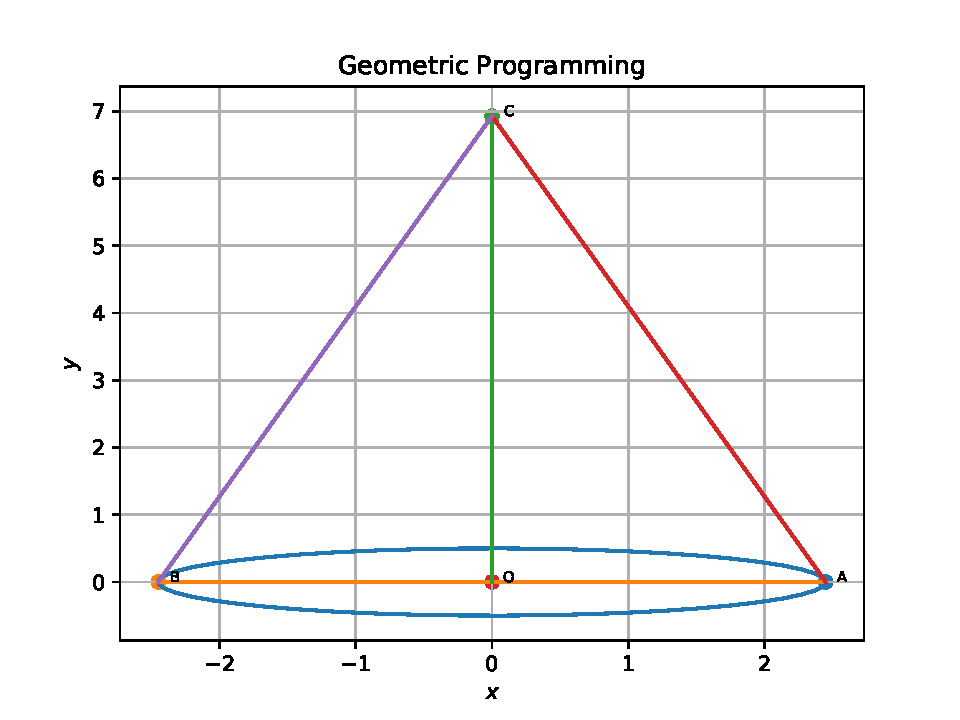
\includegraphics[width=\columnwidth]{figs/problem26.pdf}
	\end{center}
\caption{}
\label{fig:Fig1}
\end{figure}
\end{enumerate}
\end{document}
